% !TEX root = thesis.tex
\chapter{深層学習の成果とアルゴリズム}
深層学習は、MLPのうち、普通隠れレイヤーが2つ以上のものをいう。2006年にHintonらによって、レイヤーの多いニューラルネットワークを効率よく学習させる方法が発見され、発展への道が開けた\cite{hinton2006a-fast, hinton2006reducing}。深層学習では、従来よりも多くのレイヤーを扱うことで、より複雑な関数を学習できるようになった。深層学習は、数々の分類タスクにて、従来手法を大きくしのぐ成果を収め、注目を浴びている。この章では、深層学習で使われているアルゴリズムの詳細について述べる。
\section{深層学習の成果}
2012年には、GoogleがSupervisionと題してYoutubeビデオの静止画を使って多層ニューラルネットワークの教師なし学習を行わせ、結果として、猫を認識するユニットや人を認識するユニットを学習させることに成功した。また、ImageNet Large Scale Visual Recognition Competition(ILSVRC)というデータセット\cite{deng2009imagenet:}の分類にて、最先端の結果を残した\cite{le2012building}。ImageNet\footnote{\url{http://www.image-net.org/}}とは、WordNet\footnote{\url{http://wordnet.princeton.edu/}}を真似して作られたデータセットである。2009年より、100を超える様々な論文にて、画像認識のベンチマークに利用されてきている\footnote{\url{http://www.image-net.org/about-publication}}。図\ref{c3_imagenet}は、ImageNetの画像の例である。画像はツリー状に分類されており、例えば上を見ると、mammal(哺乳類)→palcental(胎盤)→carnivore(肉食)→canine(イヌ科)→dog(イヌ)→working dog(盲導犬やそり犬など使役される犬)→husky(ハスキー)というように、徐々に分類が細かくなっていくことがわかる。また、一つのカテゴリーには、9枚の画像がひもづけられている。\par
\begin{figure}[tbp]
 \begin{center}
  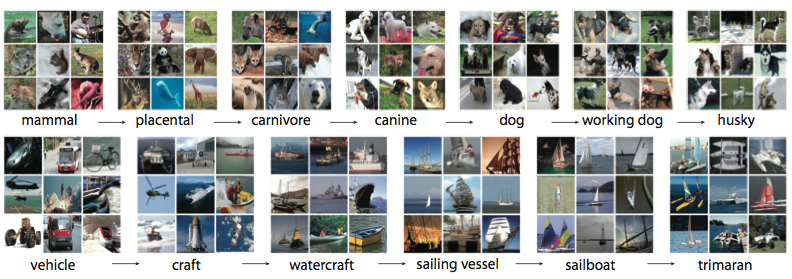
\includegraphics[width=120mm]{img/c3/imagenet}
 \end{center}
 \caption{Imagenetの画像とラベル構造の例(\cite{deng2009imagenet:}より引用)}
 \label{c3_imagenet}
\end{figure}
また、図\ref{c3_krizhevsky}は、Krizhevskeyらによる、深層学習を用いた画像分類の例である\cite{krizhevsky2012imagenet}。分類ラベルの付け方を見ると、画像の分類に失敗している場合でも、その画像に似ているものを選んでおり、人間にも理解しやすい間違い方をしていることがわかる。\begin{figure}[tbp]
 \begin{center}
  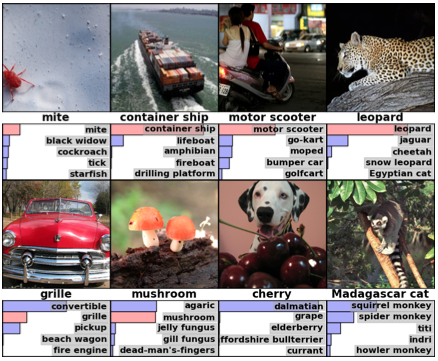
\includegraphics[width=120mm]{img/c3/krizhevsky}
 \end{center}
 \caption{深層学習による画像分類の結果の例(\cite{krizhevsky2012imagenet}より引用)}
 \label{c3_krizhevsky}
\end{figure}

深層学習は画像分析だけでなく、自然言語処理の分野でも有効なことがわかっている。Googleが公開している"word2vec"というライブラリを使うと、入力されたテキスト文書から、単語のベクトル化やクラスタリングを行うことができる\cite{mikolov2013efficient}\cite{mikolov2013linguistic}。このベクトル化により、
\begin{equation}
vector('Paris') - vector('France') + vector('Italy') = vector('Rome')
\end{equation}
\begin{equation}
vector('king') - vector('man') + vector('woman') = vector('queen')
\end{equation}
のような計算が行えるようになった。word2vecによるベクトル生成はウェブアプリにもなっており、誰でもブラウザ上でテキストデータを入れるだけで、意味ベクトルを生成できるようになっている\footnote{\url{https://code.google.com/p/word2vec/}}。word2vecでは、入力されたテキストデータから、まず単語の辞書を作り出す。次にそれぞれの単語の意味をベクトル化していく。単語を表すベクトル値を使えば、先に示した数式のような加減算を行ったり、単語同士の類似度を計測したり、クラスタリングで似た単語を仲間分けすることができる。なお、ベクトル化の計算を行う過程で、全ての単語同士の内積の和を計算していたところを止め、数個だけサンプルを取って計算することで、計算時間が短縮できるだけでなく、分類精度まで向上することが判明した\cite{mikolov2013distributed}。\par
word2vecを応用した研究も出現している。Deep Visual-Semantic Embedding model(DeViSE)\cite{frome2013devise:}と名付けられたシステムでは、zero-shot learningと呼ばれる問題を解かせるため、Supervisionとword2vecを組み合わせている。zero-shot learningとは、訓練時に一度も見たことがないクラスの画像に対し、正しく分類を行えるかという問題である。この研究では、1000カテゴリの画像による訓練を行っただけで、まだ見たことが無い20000カテゴリに属する画像を適切にラベリングしている。画像以外に全く情報がなければ分類は不可能なので、Wikipediaのテキスト内容を補助データとして使っているが、これはWordNetや意味データベースの情報を直接用いていた従来の研究\cite{mensink2012metric}\cite{rohrbach2011evaluating}\cite{palatucci2009zero-shot}に比べて、より生データに近い情報で処理に成功していると言える。\par
\begin{figure}[tbp]
 \centering
  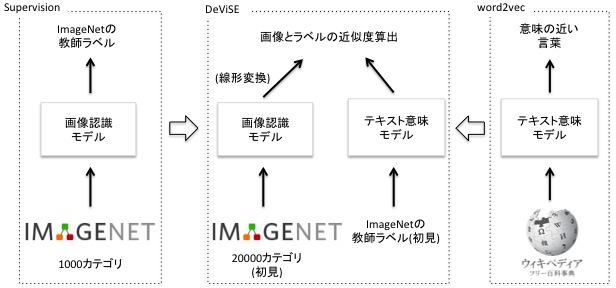
\includegraphics[width=120mm]{img/c3/devise}
 \caption{DeViSEの学習方法(\cite{frome2013devise:}を基に作成)}
 \label{c3_devise}
\end{figure}
図\ref{c3_devise}は、DeViSEの学習方法を示している\footnote{ImageNetとWikipediaのロゴは、それぞれの公式ウェブページより引用した。\url{http://www.image-net.org/splash/logo.jpg}, \url{http://upload.wikimedia.org/wikipedia/commons/a/ad/Wikipedia-logo-v2-ja.png}}。DeViseでは、画像データを意味付けするためにSupervisionを使い、Wikipediaの情報処理にword2vecを用いている。まずSupervisionにImageNetのデータを、word2vecにWikipediaのデータを与えて学習させたあと、実際の画像及び未見カテゴリのラベルを与え、画像とラベルの意味ベクトルが、出来るだけ近くなるように分類している。\par
深層学習を強化学習(reinforced learning)と組み合わせることで、ゲームを上手くプレイできるAIを作る研究も成功している\cite{mnih2013playing}。強化学習では、環境に対してAIが行動を起こし、環境から得られる報酬を最大化できるように、アルゴリズムを修正していく。多くの場合、「行動と報酬の間に時間差があり、どの行動が報酬に結びついたのか分かりにくい」「行動によって環境が変化しててしまうため、分析が難しい」といった状況設定がなされる。また、バンディット問題(Bandit Problem)というカテゴリでは、スロットゲームを題材にして、「知識を活用すると報酬は上がるが、もっと良い行動があるかもしれない」「行動の探索を優先すると、既存知識は活かせず、一時的な報酬は下がりやすい」というジレンマの解決が研究されている\cite{cesa-bianchi2013a-gang}。\cite{mnih2013playing}の研究では、ゲーム内のキャラクターをAIで行動させ、報酬としてのスコアを最大化させるような行動を学習させる。ここで深層学習は、ゲーム内の状況をモデル化して、そこから最適な行動を導き出すために用いられている。

\section{深層学習のアルゴリズム}
\subsection{Deep Belief Network}
最初にMLPの学習のブレイクスルーとなったのは、2006年のHintonらによる深層信念ネットワーク(Deep Belief Network、以下DBN)\cite{hinton2006a-fast, hinton2006reducing}である。このモデルについて解説する。
\subsubsection{教師無しpretrainingとfinetuning}
この研究では、MLPの重みをランダムに初期化した後、すぐバックプロパゲーション学習にかけるのではなく、各レイヤーの重みをあらかじめ教師無し学習で調整するアイデアが使われた。これにより、隠れ層が効率の良い素性を学習できるようになった。この教師無し学習のことを、pretrainingと呼び、バックプロパゲーションにて学習する段階の方は、finetuningと呼ぶ。pretrainingの段階では、入力側から1レイヤーずつ学習を行い、学習済のレイヤーは固定して動かさない(layer-wise greedy pretraining)。finetuningの段階では、全てのレイヤーをバックプロパゲーションにて同時に変化させていく。DBNの構造を、図\ref{c3_dbn}に示す。\par
\begin{figure}[tbp]
 \centering
  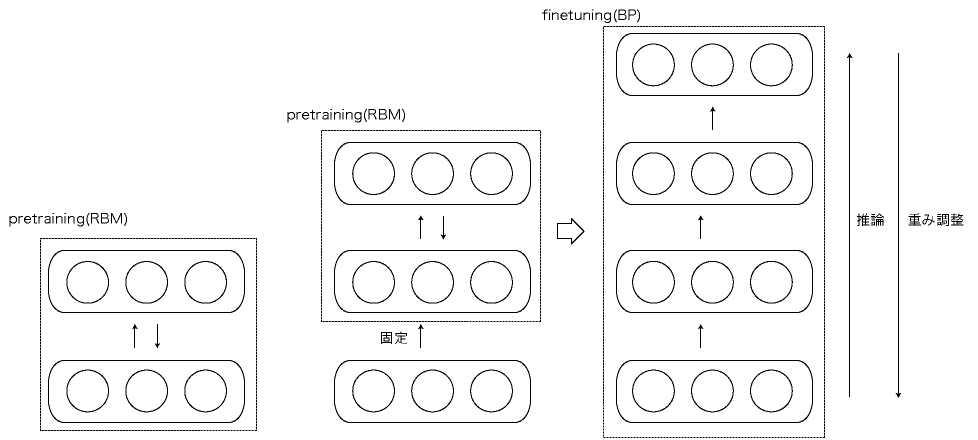
\includegraphics[width=120mm]{img/c3/dbn}
 \caption{Deep Belief Networkの構造と、学習過程 (\cite{hinton2006a-fast, hinton2006reducing}を基に作成)}
 \label{c3_dbn}
\end{figure}
教師無しpretrainingをどのような基準で行うかが問題だが、この研究では、制限付きボルツマンマシン(Restricted Boltzman Machine、以下RBM)というモデルを用いている。RBMとは、ニューラルネットワークの一種で、可視変数層と隠れ変数層の2つのレイヤーから成り立っている。RBMについては後に詳しく述べるが、DBNにおいては可視変数=入力データと考えておけばよい。RBMモデルの学習を進めることで、入力データ→隠れ変数への推論モデルを得ることができる。これが深層学習の最大の特徴の1つである、「抽象度の高い素性への変換方法自体を学習する」ことに対応している。DBNでは、RBMを1レイヤーずつ学習させながら、RBM同士を「前のレイヤーの隠れ層 = 次のレイヤーの入力層」となるようにつなげていく。これにより「入力層→抽象度の低いレイヤー→...→抽象度の高いレイヤー→出力」という、複数の隠れ層をもつDeepな構造を作り、上手くpretrainingさせることに成功している。RBMを積み重ねた最も上のレイヤーに、普通の線形レイヤーを1つ置いて、「最も抽象度の高い素性→出力値」の推測を行わせることが多い。なお、finetuningにおけるバックプロパゲーションでは、RBMにあった「隠れ層→入力層」の方のつながりは、最終レイヤーにおける誤差に影響しない。よって、以前からあるfeed-forward(前向き伝播)なMLPと同様に学習させることができる。
\subsubsection{制限付きボルツマンマシン}
DBNのpretrainingに用いられるRBMについて、少し詳しく説明する。RBM\cite{rumelhart1986parallel}は、ニューラルネットワークを用いた生成モデルの一種である。そこでまず、生成モデルについて説明した後、改めてRBMについて述べる。\par
クラス分類問題を確率的アプローチで解く方法は、生成モデル(generative model)と識別モデル(判別モデル、discriminative model)の2つに大別できる\cite{bishop2006pattern}\footnote{確率モデルを介さず、入力からクラスを得る識別関数を直接導くことも出来る。}。クラス分類問題では、まずクラス事後確率$p(C_k|x)$を各クラス$k$に対して求める。基本的には入力$x$に対して最もクラス事後確率が大きくなったクラスに分類することになる\footnote{医療における誤診断など、誤分類のタイプに応じて重要度が異なる場合、損失関数(loss function)を導入することもある。}。識別モデルでは、クラス事後確率$p(C_k|x)$のみを直接学習するのに対し、生成モデルでは、まずクラスの条件付き密度$p(x|C_k)$を学習する。これと、別途求めたクラスの事前確率$p(C_k)$を用いることで、クラス事後確率は
\begin{equation}
p(C_k|x) = \frac{p(x | C_k)p(C_k)}{p(x)} = \frac{p(x | C_k)p(C_k)}{\sum_{k}p(x | C_k)p(C_k)}
\end{equation}
によって求められる。これは、入力とクラスの同時確率$p(C_k, x)$を求めることと等価である。生成モデルの利点は、クラス分類のモデルだけでなく、入力データの性質に関する情報をも同時に得られる点にある。しかし、一般に識別モデルよりも複雑で困難な問題を解く必要が生じるため、常に生成モデルが用いられるわけではない。\par
\begin{figure}[tbp]
 \centering
  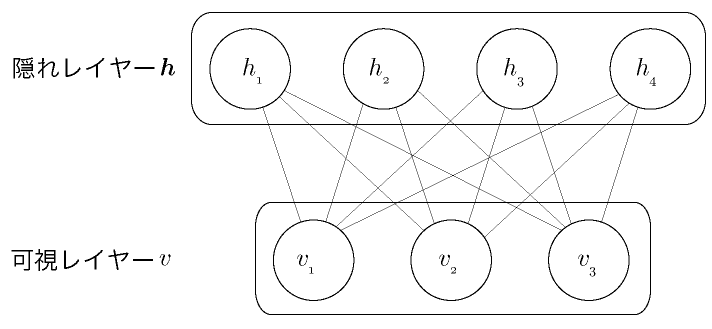
\includegraphics[width=100mm]{img/c3/rbm}
 \caption{Restriceted Boltzman Machineのネットワーク構造}
 \label{c3_rbm}
\end{figure}
さて、前述したように、RBMは可視層と隠れ層の2レイヤーで構成されるニューラルネットワークである。RBMの構造を、図\ref{c3_rbm}に示す。入力層の各ユニットの値を$v_j$, 隠れ層の各ユニットの値を$h_i$とおく。これらをまとめたベクトルをそれぞれ$\bm{v}=\{v_1, v_2, ...\}, \bm{h}=\{h_1, h_2, ...\}$とおく。これは、例えば$\bm{v}$が画像や音声などの入力データをベクトル化したもので、$\bm{h}$がこれらの変数の関係を説明する変数だと考えれば良い。ただし、$\bm{h}$が即$\bm{v}$のクラス分類に対応するとは限らないことに注意する。RBMの学習を進めると、$p(\bm{v}|\bm{h})$と$p(\bm{h}|\bm{v})$との、2方向の条件付き確率のモデルが同時に得られる。\par
RBMの学習は、自由エネルギー(Free Energy)と呼ばれる従属変数を最小にするように行われる\footnote{自由エネルギーという呼び名は、物理学から採られている。}。ここでは、最も簡単な、$v_j, h_i\epsilon\{0,1\}$のケースについて述べる。Wをvとhの間の重み、bとcを、それぞれvとhに対応するバイアス項とする。このとき、RBMにおける自由エネルギー$F(v)$は、
\begin{equation}
F(v) = -b' v-\sum_{i}log(1+e^{(c_i+W_{i}v)})
\end{equation}
となる。この自由エネルギーを、SGDなどのアルゴリズムを用いて最小化することで、目標となる生成モデルを得ることができる。なお、自由エネルギーの導入と最小化というアプローチは、エネルギーに基づくモデル(エネルギーに基づくモデル)と呼ばれるアルゴリズム群に共通して用いられる概念であり、自由エネルギーにもさらに様々なモデルで使える一般的な定義が存在するが、割愛する。
\subsubsection{DBNの性能}
Hintonらによる最初のDBN研究では、評価実験としてMNISTの手書き数字認識データセットを用いている。彼らは各レイヤーのユニット数が"784-500-500-2000-10"という構造のDBNによって、学習を行った。そして、順序不変(Permutation Invariant)と呼ばれるタスクにて、当時の最先端記録を塗り替えたことにより、注目された。ここで、順序不変とは、データを単なる1次元の値の集まりと見なし、2次元の画像という事前情報の利用を禁止した状態で、分類実験を行うことである。具体的には、画像的変形によるデータの水増しや、2次元的畳み込み(\ref{subsec:c3_cnn}節にて詳述)などが当てはまる。順序不変の制約下で良い成果を出したDBNは、画像の性質を利用した畳み込みネットワークに比べたとき、画像以外の1次元のデータに対しても適用しやすいアルゴリズムだと考えられる。

\subsection{Stacked Denoising Autoencoder}
DBNと共に、1次元のデータに対して広く用いることができるモデルが、Stacked Denoising Autoencoder(以下SDA)である。これは2007年に提唱されたAutoencoder\cite{bengio2007greedy}というモデルを基に、2008年に発表された\cite{vincent2008extracting}。基本的なアイデアは、DBNにおけるRBMを、Denoising Autoencoder(以下DA)という別のモデルに変更することである。
\subsubsection{Autoencoder}
DAは、Autoencoderの特殊なバージョンなので、まずはAutoencoderについて説明する。Autoencoderは、ニューラルネットワークの一種であり、入力されたデータを再現するようなモデルを学習する。\cite{bourlard1988auto, hinton1994autoencoders, schwenk1995transformation}\par
Autoencoderの構造を、\ref{c3_autoencoder}に示す。Autoencoderは、この図でいうInput, Representation, Outputの3つのレイヤーから構成されている。OutputとInputの値が一致するように、重み$W$と$W'$を学習させていく。この一致に成功しているとき、「
RepresentationはInputを復元(decode)するための情報を含んでいる」、つまり「RepresentationはInputの別表現である」と考えられる。Inputに与えられたデータを、別の素性を用いたRepresentationに符号化(encode)していることから、自分自身の符号化方法を覚えるという意味で、Autoencoderという名前がつけられている。\par
Autoencoderを用いることで、Inputを別の素性に変換することができる。しかし一方で、必ずしも得られた素性が抽象度の高いものになっているとは限らない。例えば、最も自明なAutoencoderは、EncoderとDecoderの双方に恒等写像を用いることである。恒等写像は入力値に一切の影響を与えないため、InputとRepresentationとOutputの値は一致し、確かにReconstruction Errorは0になる。しかし、InputとRepresentationの抽象度は同じであり、素性学習としての有用性は全くない。\footnote{実用上は、SGDを用い、入力レイヤーよりも表現レイヤーのユニット数を多くとり、非線形な関数をEncoderやDecoderに使うことで、抽象度が高くスパースな素性が獲得されることがわかっている\cite{bengio2007greedy}\cite{lee2007sparse}。しかし、理論的証明はされていない。}この素性学習の不確実性の問題を緩和するのが、次に述べるDAである。
\begin{figure}[tbp]
 \begin{center}
  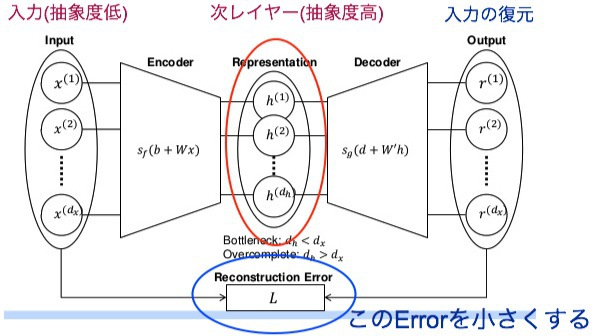
\includegraphics[width=80mm]{img/c3/autoencoder}
 \end{center}
 \caption{Autoencoderの構造図}
 \label{c3_autoencoder}
\end{figure}

\subsubsection{Denoising Autoencoder}
DAは、Autoencoderを拡張したものである。Input層に渡す入力データの一部をランダムに隠し(corrupted input)、元の隠されていない入力データを復元するように学習させる。データを隠す割合をcorruption rateといい、例えばcorruption rateが30\%の場合、100次元の画像データを入力すると、そのうち30次元分をランダムに選んで、数値を0にしてしまうことになる。図\ref{c3_da_pic}は、DAが働く様子を、画像の入力レイヤーの場合について表している。\par
また、図\ref{c3_da}は、元の入力データ群から外れた入力データを作り、これを復元している様子を模式的に表している。データの一部を隠すことによって、より頑堅な素性の作り方のモデルを得ることが出来ると考えられている。\par
なお、DAの学習過程には、RBMのようなエネルギーに基づくモデルとの類似性があることがわかっている\cite{vincent2011a-connection}。
\begin{figure}[tbp]
 \begin{center}
  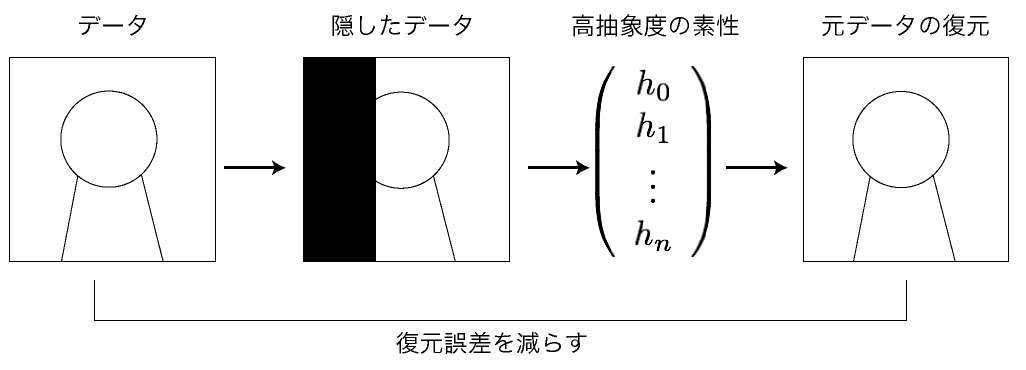
\includegraphics[width=80mm]{img/c3/da_pic}
 \end{center}
 \caption{画像に対するDenoising Autoencoder}
 \label{c3_da_pic}
\end{figure}
%様々な隠し方を図にする
\begin{figure}[tbp]
 \begin{center}
  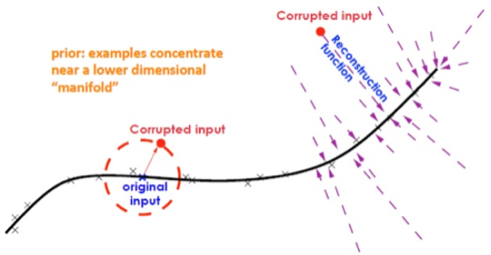
\includegraphics[width=80mm]{img/c3/da}
 \end{center}
 \caption{Denoising Autoencoderの模式図 (http://www.iro.umontreal.ca/~bengioy/talks/icml2012-YB-tutorial.pdfより引用)}
 \label{c3_da}
\end{figure}

\subsubsection{Stacked Denoising Autoencoder}
SDAは、DBNのpretrainingで、RBMの代わりにDAを用いたものである。DBN同様、前の層のRepresentationレイヤー = 次の層のInputレイヤーとなるように、DAで学習したレイヤーを積み重ねていく。最終レイヤーには、DAではなくソフトマックスレイヤーなどを置き、最終的な確率を出して、分類を行わせる。図\ref{c3_sda}は、SDAにて、どのようにpretrainingが繰り返され、DAが積み上げられていくのかを表している。いったんpretrainingが済んだら、そのレイヤーの入力は隠さず、学習された重みをそのまま使って高い抽象度の素性を作る。そして、その新しい素性を入力と捉えて、新たにDAの学習を行わせる。これを繰り返してレイヤーを積み上げ、最終的に良い素性を学習しやすいMLPを作ることで、finetuning段階でも学習がスムーズに進み、精度のよい推論ができるようになる。
\begin{figure}[tbp]
 \centering
  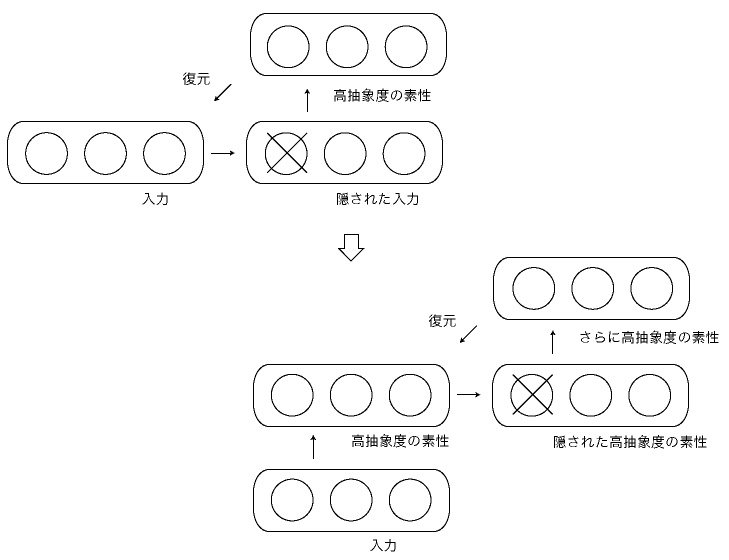
\includegraphics[width=100mm]{img/c3/sda}
 \caption{Stacked Denoising Autoencoderにおける学習の進行 (\cite{vincent2008extracting}を基に作成)}
 \label{c3_sda}
\end{figure}

%深層学習の登場 Hinton, Bengio, LeCun
%画像認識タスクでの成績、音声認識タスクでの成果、猫認識
%MNIST, CIFAR, SVHNなどにおけるconv.net、Maxout, DropConnectの優位

\subsection{Convolutional Neural Network}
\label{subsec:c3_cnn}]
Convolutional Neural Network(以下CNN)は、画像認識にて使われるニューラルネットワークの一種である。DBNやSDAのようにユニットが1対1で接続されるのではなく、画像上で距離が近いユニットを一まとめに考えるが特徴である。具体的には、フィルターと呼ばれる小さな四角形を、画像の上で動かしていき、フィルターが覆っている部分の性質を抽出して次のレイヤーに渡していく。フィルターは行列で表現されており、フィルター行列の各要素と、画像の各画素を掛け算し、その和を取ることで、次のレイヤーに渡す値が得られる。基本的な構造は、図\ref{c3_convolution}のようになっている。この図では、2回の畳み込みを行ったあと、十分に画像の素性が得られたところで、従来のMLPで見られる隠れレイヤーを1つ介して、出力を得ている。\par
\begin{figure}[tbp]
 \centering
  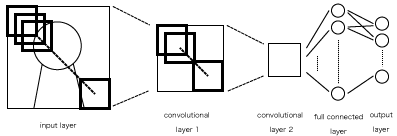
\includegraphics[width=80mm]{img/c3/convolution}
 \caption{畳み込みニューラルネットワークの仕組み}
 \label{c3_convolution}
\end{figure}
CNNの発祥はDBNやSDAよりも古い。画像上の各部分ごとに性質を抜き出しニューラルネットワークを構成するというアイデアは、人間の視覚野の仕組みを参考にしたもので、1980年のNeocognitronを始めとして\cite{fukushima1980neocognitron}\cite{fukushima1983neocognitron}様々な形で提唱されている\cite{lecun1998gradient-based}\cite{serre2007robust}。2003年に提唱されたCNNのモデルが、画像認識ベンチマークのMNISTにて、今でも5位の精度を保っており\cite{simard2003best}、2012年のものは2位となっている\cite{ciresan2012multi-column}。フィッシャーベクトルなど既存の画像認識手法との組み合わせでも、良い性能を発揮できることがわかっている\cite{nakayama2013efficient}。ここで紹介するのは、1998年にLeCunらが紹介した方法\cite{lecun1998gradient-based}であり、ほとんどのCNNに使われているアルゴリズムの基本的な部分である。
\subsubsection{Feature Map}
実際のCNNでは、Feature Mapと呼ばれる方法が使われている。これは、フィルタが1つだけでなく、複数種類のフィルタを、複数枚の画像の上で動かしていく方法である。図\ref{c3_convolution}の構造に、Feature Mapの考え方を適用すると、\ref{c3_feature_map}のようになる。この図では、フィルターが移動する様子は省略している。四角形はFeature Map1つを、円はMLPのユニット1つを表している。Feature Map同士では、フィルタによる畳み込みによって情報が伝達される。Feature MapからMLPの隠れレイヤーにつながる部分では、まず全てのFeature Mapを直列につなぎ、1次元のベクトルに並び替えて入力している。残りは、通常のMLPと同じように処理される。(なお、図\ref{c3_convolution}では、簡単のため、Feature Mapは表現されていない。)\par
1枚のmapが、1書類のフィルタに対応しているので、フィルタの数と同じだけ次のレイヤーのFeature Mapが用意されている。それぞれのフィルタを、全てのFeature Mapの上で動かして、畳み込み計算を行っていく。最終的に、普通のMLPに帰着させるところは変わらない。\par
Feature Mapは、カラー画像を扱うときにも利用できる。カラー画像データは、ほとんどの場合Red、Green、Blueの光の3原色に対応する3つの値にて表現される。これを省略してRGBと呼ぶ。畳み込みネットワークの入力レイヤーにて、画像サイズと同じ大きさの、RGBの3色に対応する3つのFeature Mapを設定することで、色情報を簡単に扱うことができる。

\begin{figure}[tbp]
 \centering
  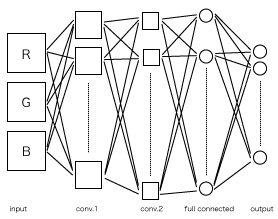
\includegraphics[width=80mm]{img/c3/feature_map}
 \caption{CNNとFeature Map}
 \label{c3_feature_map}
\end{figure}

\subsubsection{MaxPooling}
CNNにて、もう1つ広く使われている方法が、max-poolingである。max-poolingレイヤーは普通畳み込みレイヤー同士の間に置かれる。max-poolingでは、畳み込みレイヤーで得られた画素を、部分ごとにたたみ込んでいく。ただし、畳み込みレイヤーの計算に使うフィルタとは違い、重み行列は用いず、単純に対象領域の画素値のmaxを取って、次のレイヤーに渡していく。また、畳み込みレイヤーではフィルタを1ピクセルずつ動かしていくが、max-poolingレイヤーでは、一度にフィルタのサイズと同じだけ動かし、畳み込み対象領域が重ならないようにする。また、フィルタのサイズは2x2ピクセルに設定されることが多い。図\ref{c3_maxpooling}の左側は、max-poolingによる畳み込みの様子を、右側ではmax-poolingレイヤーによる畳み込みの全体の様子を表している。\par
max-poolingを用いることにより、各レイヤーの次元数を効率良く下げることが出来る。また同時に、ピクセルの位置が少し変化しても同じ結果が得られるので、位置的な頑健性(robustness)を上げることも出来る。\par
max-poolingレイヤーを併用した場合の、一般的なCNNの全体図を、図\ref{c3_convnet}に挙げる。なお、この図では、各Feature Mapごとのつながりは省略している。

\begin{figure}[tbp]
 \centering
  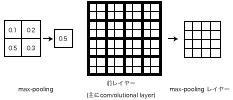
\includegraphics[width=80mm]{img/c3/maxpooling}
 \caption{max-poolingと、max-poolingレイヤーの作用}
 \label{c3_maxpooling}
\end{figure}

\begin{figure}[tbp]
 \centering
  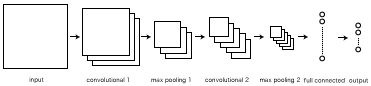
\includegraphics[width=120mm]{img/c3/convnet}
 \caption{max-poolingレイヤーを取り入れたCNN}
 \label{c3_convnet}
\end{figure}

\subsection{DropoutとDropConnect}
\label{c3_dropout}
Dropoutとは、2012年にHinton氏らによって提案された、過学習(over fitting)を防ぐための技術である\cite{hinton2012improving}。過学習とは、機械学習全般において使われる用語で、学習モデルが訓練中に見たデータへの適応を重視し過ぎたために、未知のデータをうまく識別できなくなる現象のことを指す。Dropoutでは、過学習を防ぐため、各レイヤーからの出力をランダムに消去してしまう。これによって各ユニットには、他のユニットに頼らず自力で学習をする必要が生じ、より様々な入力に対応しやすい堅固(robust)なモデルが獲得される、と考えられている。図\ref{c3_dropout_timit}は、音声認識のTIMITデータベース\cite{fisher1986the-darpa}\footnote{\url{http://catalog.ldc.upenn.edu/LDC93S1}}に対する識別精度である。Dropoutを使うことで、使わなかった場合に比べ、特に繰り返し回数(学習の繰り返し回数)が大きい場合に、分類誤差を減少出来ていることがわかる。
\begin{figure}[tbp]
 \centering
  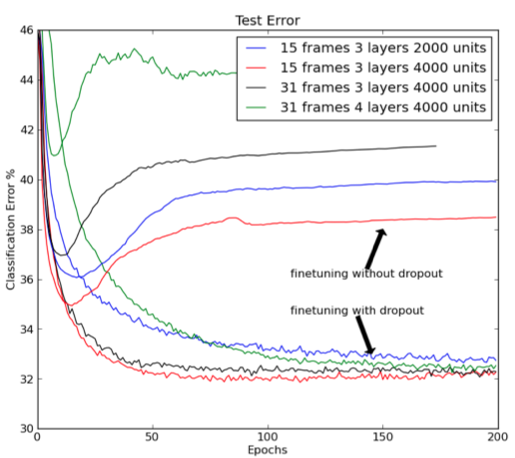
\includegraphics[width=100mm]{img/c3/dropout_timit}
 \caption{DropoutによるTIMITデータベースの識別結果 (\cite{hinton2012improving}より引用)}
 \label{c3_dropout_timit}
\end{figure}
\par
DropConnectは、Dropoutをさらに一般化した手法である。DropConnectでは、各ユニットからの出力ではなく、ユニット同士のつながりをランダムにカットしている。図\ref{c3_dropconnect}は、ニューラルネットワークにおけるニューロン同士の接続が、ランダムに切断されている様子を表している。
\begin{figure}[tbp]
 \begin{center}
  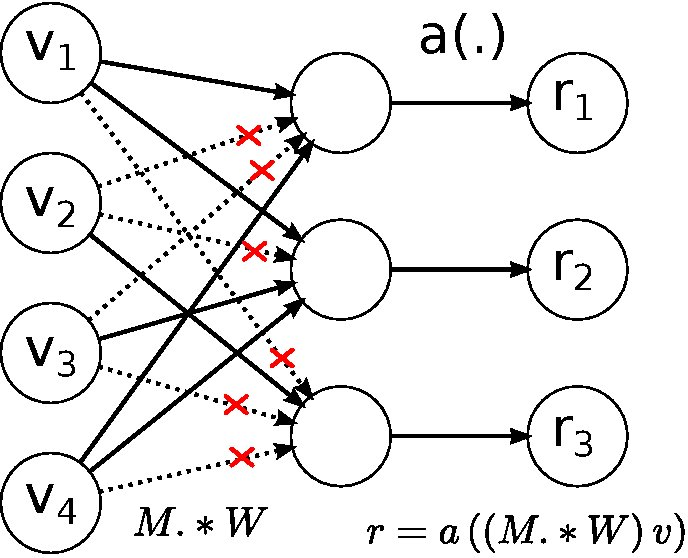
\includegraphics[width=90mm]{img/c3/nn_dc}
 \end{center}
 \caption{DropConnectの模式図(http://cs.nyu.edu/~wanli/dropc/)より引用}
 \label{c3_dropconnect}
\end{figure}

\subsection{ハイパーパラメータ}
機械学習一般でハイパーパラメータ(hyper parameter)と言えば、モデルのパラメータの中で、特にモデル全体の性質を決定するものを指す。各レイヤー間を結びつける重み行列やバイアス項も、モデルを構成する重要なパラメータであるが、個々のユニットの挙動にしか影響しないため、ハイパーパラメータとは呼ばれない。以下に、ニューラルネットワークにおけるハイパーパラメータの一例を挙げる。
\begin{itemize}
\item \textbf{隠れレイヤー数} 入力レイヤーと出力レイヤーの間に、どのようなレイヤーをいくつ挟むか。深層学習の出現以前は、実用的なニューラルネットワークの隠れレイヤー数は1つのみだった。このパラメータはモデル選択とも密接に絡んでいる。
\item \textbf{隠れレイヤーのユニット数} 各レイヤーが含むユニット数はいくつにするか。
\item \textbf{学習率} BPによって伝わってきた誤差を、どの程度パラメータに反映させるか。普通1に近い値にする。また、訓練の反復数が進むにつれて、線形的・指数的・階段状など様々なやり方で学習率を減少させていくこともある。
\item \textbf{慣性率} BPを繰り返す過程で、前回のBPによる重み修正の値を、もう一度適用することで、平均化のような効果が得られることがわかっている。「前回の重み修正値の影響」を表す項を慣性項と呼んでおり、この慣性項にかかる、慣性の効きの強さを表す係数のことを慣性率と呼ぶ。適切な初期値と慣性項の組み合わせは、学習性能の向上をもたらすとわかっている\cite{sutskever2013on-the-importance}。
\item \textbf{停止条件} 訓練段階をいつ停止するか。例えば、「規定回数の訓練を行ったら、訓練を停止する」という条件の場合、訓練の回数(Epoch数)がハイパーパラメータである。「訓練によるモデル変化が一定未満になったら停止する」というアルゴリズムの場合、停止を決めるためのモデル変化の閾値がハイパーパラメータである。
\item \textbf{corruption rate} SDAにおける、入力のcorruption rateも、ハイパーパラメータの内に含まれる。
\end{itemize}
ハイパーパラメータは、モデルの学習効率を左右する非常に重要な値である。学習性能を高めるためには、ハイパーパラメータの適切な値を決める方法が必要である。しかし深層学習では、ハイパーパラメータの個数が多くなる傾向があり、その調整は難しい。ハイパーパラメータを決める方法としては、SVMの学習でよく用いられるGrid Search法が広く知られている\cite{hsu2003a-practical}。これは、各ハイパーパラメータ毎に数個の候補値を決め、それらの組み合わせを全探索することで、最も学習性能の高いハイパーパラメータの候補値の組み合わせを決定する方法である。候補値の組み合わせをハイパーパラメータ空間上にプロットすると、複数の格子点で升目状の模様が描かれる様子から、Grid Searchの名が付いている。パラメータ候補値の決め方、つまり格子点の打ち方は、ヒューリスティックに決められる。SVMでよく用いられるRBFカーネルでは、ハイパーパラメータが2つしかなく、この場合Grid Searchは非常に有効とされている\footnote{LIBSVMには、grid.pyというGrid Search用のスクリプトが付属している。}。一方、\cite{bengio2012practical}によれば、深層学習ではGrid SearchよりもRandom Searchの方が性能が優れているとされている。しかし、同時に小規模なGrid Searchや手作業による調整も未だ有用であり、さらに効率の良いハイパーパラメータ探索法も求められている。

\subsection{活性化関数}
各ユニットに入力された値は、ある一定の関数によって増幅・変換される。これは人間の神経細胞を真似た仕組みで、神経細胞の化学物質による活性化にちなんで、活性化関数(activation function)と呼ばれる。この項では、ニューラルネットにおける様々な活性化関数を紹介する。
\subsubsection{ヘビサイド関数}
始めにニューラルネットワークの活性化関数として用いられたがヘビサイドの階段関数である。この関数は負値に0、正値に1を返す。これを数式で表すと、
\begin{equation}
H(x)= \left\{\begin{array}{cc} 0\quad (x < 0)\\ 1 \quad (x > 0)\end{array}\right.
\end{equation}
となる。ただし、これだけでは$x=0$の点で不連続になるので、$H(x)=0$や$H(x)=0.5$などの定義が用いられる。ヘビサイド関数のグラフを\ref{c3_heaviside}に示す。\par
ヘビサイド関数は、ニューロンが受けた刺激の総和を測り、閾値を超えていれば次のニューロンにも情報を伝達し、超えていなければ何もしないという性質を、そのまま表現している。しかし、この関数は微分不可能なため、バックプロパゲーションを行う上では不都合であり、特に深層学習のネットワークモデルにおいて使われることは少ない。
\begin{figure}[tbp]
 \centering
  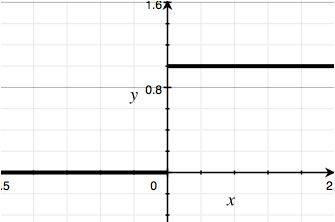
\includegraphics[width=80mm]{img/c3/heaviside}
 \caption{ヘビサイドの階段関数}
 \label{c3_heaviside}
\end{figure}

\subsubsection{シグモイド関数と双曲線正接関数}
シグモイド関数は、ヘビサイド関数に似ているが、全域にて非線形かつ微分可能である。非線形関数を用いることでニューラルネットワークの表現力が増し、微分可能なのでバックプロパゲーションに適している。この2つの長所により、ニューラルネットワークの活性化関数として良く用いられる。以下の式で表される。%citation needed
\begin{equation}
S(x) = \frac{1}{1+e^{-x}}
\end{equation}
また、微分した形が同じシグモイド関数で表されるという特徴があり、実装も容易である。
\begin{eqnarray}
\frac{d}{dx}S(x) &=& \left( \frac{1}{1+e^{-x}} \right) \left( \frac{-e^{-x}}{1+e^{-x}} \right)\\
&=& S(x)(1-S(x))
\end{eqnarray}
シグモイド関数のグラフが図\ref{c3_sigmoid}である。ヘビサイド関数を$x=0$の付近のみ滑らかにしたような形をしている。この関数は、xの絶対値が大きくなるにつれ、yの変化が非常にに小さくなっている。そのため、ユニット間伝達において、入力と重みの積が大きくなってしまうと、その部分は誤差のバックプロパゲーションに対する反応が小さくなってしまい、学習が進みにくくなってしまうという弱点がある。%citation needed
\begin{figure}[tbp]
 \centering
  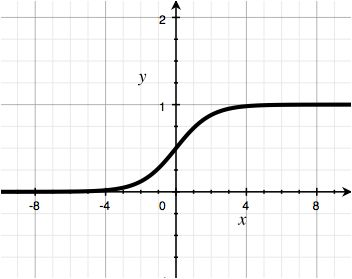
\includegraphics[width=80mm]{img/c3/sigmoid}
 \caption{シグモイド関数}
 \label{c3_sigmoid}
\end{figure}
また、活性化関数としてシグモイド関数と同等によく使われる関数に、双曲線正接関数、通称tanh関数がある。シグモイド関数とtanh関数は線形の差しかないため、ニューラルネットワークの性能という面では、どちらを使用しても等価である。
\begin{equation}
tanh(x) = \frac{e^x-e^{-x}}{e^x+e^{-x}} \\\\
\end{equation}
\begin{equation}
S(x) = \frac{tanh(x/2)+1}{2}
\end{equation}

\subsubsection{整流関数}
整流関数(rectifier function)は、最近のニューラルネットワークにおいてよく用いられている活性化関数である。この関数を用いたユニットを、整流ユニット(Rectifier Linear Unit、以下ReLU)と呼ぶ。図\ref{c3_rectifier}は、整流関数のグラフである。
\begin{equation}
f(x) = max(0, x) = \left\{\begin{array}{cc} 0\quad (x < 0)\\ x \quad (x > 0)\end{array}\right.
\end{equation}
ReLUの使用は深層ニューラルネットワークの性能向上につながるとされているが、その理由はまだ解明されていない。%citation needed

\begin{figure}[tbp]
 \centering
  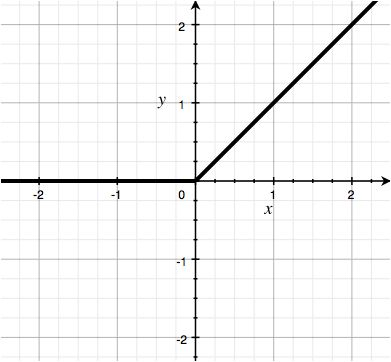
\includegraphics[width=80mm]{img/c3/rectifier}
 \caption{整流関数}
 \label{c3_rectifier}
\end{figure}

\subsubsection{Maxout}
Maxout Networkとは、バックプロパゲーションを伴う単純な多層MLP構造に、\ref{c3_dropout}で述べたDropout法を組み合わせ、さらにMaxoutユニットという、特殊な活性化関数を含むユニットを用いたニューラルネットワークである\cite{goodfellow2013maxout}。Maxout Networkの1レイヤー分の構造を、図\ref{c3_maxout_arch}に示す。\par
Maxoutユニットでは、複数の線形ユニットの出力をまとめ、その最大値のみを取っている。これにより、任意の凸関数を近似することが出来る。図\ref{c3_maxout_app}は、Maxoutユニットが凸関数を近似する様子を、1次元の入力について示している。そして、複数のMaxoutユニットの線形和を取ることは、複数の近似された凸関数の線形和を取ることである。これによって、最終的に任意の連続関数を近似できることが証明されている。%近似の説明
\begin{figure}[tbp]
 \begin{center}
  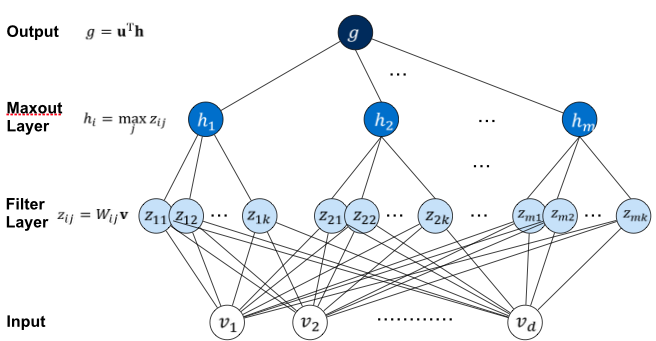
\includegraphics[width=100mm]{img/c3/maxout_arch}
 \end{center}
 \caption{Maxout Networkの構造図}
 \label{c3_maxout_arch}
\end{figure}
\begin{figure}[tbp]
 \begin{center}
  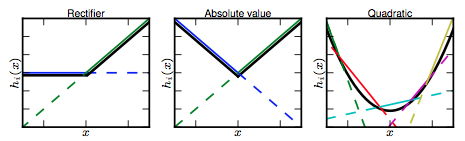
\includegraphics[width=130mm]{img/c3/maxout_app}
 \end{center}
 \caption{Maxoutユニットが1次元凸関数を近似する様子(\cite{goodfellow2013maxout}より引用)}
 \label{c3_maxout_app}
\end{figure}
